\documentclass[aspectratio=169,xcolor={dvipsnames,table}]{beamer}
\usepackage[no-math,deluxe,haranoaji]{luatexja-preset}
\renewcommand{\kanjifamilydefault}{\gtdefault}
\renewcommand{\emph}[1]{{\upshape\bfseries #1}}
\usetheme{metropolis}
\metroset{block=fill}
\setbeamertemplate{navigation symbols}{}
\setbeamertemplate{blocks}[rounded][shadow=false]
\usecolortheme[rgb={0.7,0.2,0.2}]{structure}
%%%%%%%%%%%%%%%%%%%%%%%%%%%
%%%%%%%%%%%%%%%%%%%%%%%%%%%
%% さまざまなアイコン
%%%%%%%%%%%%%%%%%%%%%%%%%%%
%\usepackage{fontawesome}
\usepackage{fontawesome5}
\usepackage{figchild}
\usepackage{twemojis}
\usepackage{utfsym}
\usepackage{bclogo}
\usepackage{marvosym}
\usepackage{fontmfizz}
\usepackage{pifont}
\usepackage{phaistos}
\usepackage{worldflags}
\usepackage{jigsaw}
\usepackage{tikzlings}
\usepackage{tikzducks}
\usepackage{scsnowman}
\usepackage{epsdice}
\usepackage{halloweenmath}
\usepackage{svrsymbols}
\usepackage{countriesofeurope}
\usepackage{tipa}
%%%%%%%%%%%%%%%%%%%%%%%%%%%
\usepackage{tikz}
\usetikzlibrary{calc,patterns,decorations.pathmorphing,backgrounds}
\usepackage{tcolorbox}
\usepackage{tikzpeople}
\usepackage{circledsteps}
\usepackage{xcolor}
\usepackage{amsmath}
\usepackage{booktabs}
\usepackage{chronology}
\usepackage{signchart}
%%%%%%%%%%%%%%%%%%%%%%%%%%%
%% 場合分け
%%%%%%%%%%%%%%%%%%%%%%%%%%%
\usepackage{cases}
%%%%%%%%%%%%%%%%%%%%%%%%%%
\usepackage{pdfpages}
%%%%%%%%%%%%%%%%%%%%%%%%%%%
%% 音声リンク表示
\newcommand{\myaudio}[1]{\href{#1}{\faVolumeUp}}
%%%%%%%%%%%%%%%%%%%%%%%%%%
%% \myAnch{<名前>}{<色>}{<テキスト>}
%% 指定のテキストを指定の色の四角枠で囲み, 指定の名前をもつTikZの
%% ノードとして出力する. 図には remember picture 属性を付けている
%% ので外部から参照可能である.
\newcommand*{\myAnch}[3]{%
  \tikz[remember picture,baseline=(#1.base)]
    \node[draw,rectangle,line width=1pt,#2] (#1) {\normalcolor #3};
}
%%%%%%%%%%%%%%%%%%%%%%%%%%
%% \myEmph コマンドの定義
%%%%%%%%%%%%%%%%%%%%%%%%%%
%\newcommand{\myEmph}[3]{%
%    \textbf<#1>{\color<#1>{#2}{#3}}%
%}
\usepackage{xparse} % xparseパッケージの読み込み
\NewDocumentCommand{\myEmph}{O{} m m}{%
    \def\argOne{#1}%
    \ifx\argOne\empty
        \textbf{\color{#2}{#3}}% オプション引数が省略された場合
    \else
        \textbf<#1>{\color<#1>{#2}{#3}}% オプション引数が指定された場合
    \fi
}
%%%%%%%%%%%%%%%%%%%%%%%%%%%
%%%%%%%%%%%%%%%%%%%%%%%%%%%
%% 文末の上昇イントネーション記号 \myRisingPitch
%% 通常のイントネーション \myDownwardPitch
%% https://note.com/dan_oyama/n/n8be58e8797b2
%%%%%%%%%%%%%%%%%%%%%%%%%%%
\newcommand{\myRisingPitch}{
\begin{tikzpicture}[scale=0.3,baseline=0.3]
\draw[->,>=stealth] (0,0) to[bend right=45] (1,1);
\end{tikzpicture}
}
\newcommand{\myDownwardPitch}{
\begin{tikzpicture}[scale=0.3,baseline=0.3]
\draw[->,>=stealth] (0,1) to[bend left=45] (1,0);
\end{tikzpicture}
}
%%%%%%%%%%%%%%%%%%%%%%%%%%%%
%\AtBeginSection[%
%]{%
%  \begin{frame}[plain]\frametitle{授業の流れ}
%     \tableofcontents[currentsection]
%   \end{frame}%
%}

\usepackage{highlightx}
\usetikzlibrary{positioning, decorations.pathreplacing, calc}
%%%%%%%%%%%%%%%%%%%%%%%%%%%
% --- Color Customization (Urban Night Theme) ---
% Deep Midnight Blue for background
\definecolor{CityNight}{HTML}{0B1021} 
% Vibrant Cyan for accents/structure% Vibrant Cyan for accents/structure
\definecolor{NeonCyan}{HTML}{00F0FF}
% Soft White for text
\definecolor{CloudWhite}{HTML}{F0F0F0}
% Muted gray for table rows
\definecolor{TableRowOdd}{HTML}{161B33}
\definecolor{TableRowEven}{HTML}{0B1021}

% --- Font Setup ---
% Metropolis uses Fira Sans by default if compiled with XeLaTeX/LuaLaTeX.
% Ensure fonts are readable.
\usefonttheme{professionalfonts}
%%%%%%%%%%%%%%%%%%%%%%%%%%
\title{English is fun.}
\subtitle{When do you play baseball?}
\author{}
\institute[]{}
\date[]

%%%%%%%%%%%%%%%%%%%%%%%%%%%%
%% TEXT
%%%%%%%%%%%%%%%%%%%%%%%%%%%%
\begin{document}
\begin{frame}[plain]
  \titlepage
\end{frame}

\section*{授業の流れ}
\begin{frame}[plain]
  \frametitle{授業の流れ}
  \tableofcontents
\end{frame}

%%%%%%%%%%%%%%%%%%%%%%%%%%%%%%%
\section{when \textipa{/w\'en/}}
\subsection{When is your birthday?: be動詞のとき}
\begin{frame}[plain]{~はいつ?}
be動詞のとき

\mbox{}\hspace{55pt}Your birthday is  \alt<3->{\myAnch{FOCUS}{NavyBlue}{August 7th}}{\myAnch{focus}{white}{August 7th}}.%
\hfill{\scriptsize August \textipa{/\'\textopeno :g@st/} 8月}

\pause


\vspace{7pt}

\mbox{}\hfill{}{\small cf. \myEmph[5-]{Maroon}{Is your birthday} August 7th? \scalebox{1.1}{\myRisingPitch}}%

\vspace{-5pt}

\hfill{\scriptsize Yes/Noで答える疑問文}

\visible<4->{\myAnch{wh}{NavyBlue}{When} \myEmph[5-]{Maroon}{is your birthday} ?}%\myAnch{question}{orange}{?}}
\visible<6->{\scalebox{1.4}{\myDownwardPitch}}

\pause

%\mbox{}\hspace{30pt}\myAnch{txt1}{white}{\small 先頭にWho}

\visible<4->{%
\begin{tikzpicture}[remember picture, overlay]
\draw[->, line width = 3pt, opacity = .5, NavyBlue] (focus.south) to[out=-90, in=90] node[sloped,above,text=black,font=\tiny,pos=.6]{Whenに置き換えて先頭へ} node[sloped,below,text=black,font=\tiny,pos=.4]{その後は疑問文の語順} (wh.north);
\end{tikzpicture}
}
\vspace{-10pt}

\begin{block}<7->{Topics for Today}\small
\begin{itemize}\setbeamertemplate{items}[square]\small
 \item<8-> 疑問詞{\bfseries when}(いつ)を先頭に置く\hfill\textipa{/w\'en/}
% \item When is 〜?「〜はいつ」
 \item<9-> {\bfseries When}の後ろは、Yes/Noで答える疑問文の語順と同じ
 \item<10->   文末に`?'をつける / イントネーションは\myDownwardPitch{}(下降調)%
\end{itemize}
     \end{block}
\hfill{\tiny 0138}\,{\scriptsize \myaudio{./audio/014_when_01.mp3}}

\end{frame}
%%%%%%%%%%%%%%%%%%%%%%%%%%%%%%%%%%%%%%%%%%%%%%
\subsection{When do you play tennis?: 一般動詞のとき}
\begin{frame}[plain]\frametitle{When do you play tennis?}
%\Large
一般動詞のとき

\pause

\mbox{}\hspace{55pt}%
You play tennis \alt<4->{\myAnch{FOCUS2}{NavyBlue}{on Sundays}}{\myAnch{focus2}{white}{on Sundays}}.

\pause

\mbox{}\hfill%
{\small cf. \myEmph[6-]{Maroon}{Do you play} tennis on Sundays? \scalebox{1.4}{\myRisingPitch}}

\vspace{-5pt}

\hfill\visible<3->{{\small Yes/Noで答える疑問文}}

\visible<5->{\myAnch{WH2}{NavyBlue}{When} \myEmph[6-]{Maroon}{do you play} tennis?}%\myAnch{question2}{orange}{?}}
\visible<7->{\scalebox{1.4}{\myDownwardPitch}}

\visible<5->{%
\begin{tikzpicture}[remember picture, overlay]
 \draw[line width = 3pt, opacity = .5, NavyBlue, ->] (focus2.south) to[out=-90, in=90] node[sloped,above,text=black,font=\tiny,pos=.6]{Whenに置き換えて先頭へ} node[sloped,below,text=black,font=\tiny,pos=.4]{その後は疑問文の語順}(WH2.north);
\end{tikzpicture}
}

\vspace{-20pt}

\begin{block}<8->{Topics for Today}
\pause
\begin{itemize}\setbeamertemplate{items}[square]\small
 \item<9-> 疑問詞{\bfseries When}を先頭に置く
 \item<10-> {\bfseries When}の後ろはYes/Noで答える疑問文の語順と同じ

\hfill{}When\,\,\,$\left\{ \begin{tabular}{l}
	do\\
	does
%	  do / does\\
%	  did\\
%	  will\\
	 \end{tabular}\right\}$%
\,\,$+$ S $+$ 原形 \ldots ? 


%\hfill{}When do you 原形 \ldots ?\\
%\hfill{}When does she 原形 \ldots ?\\
%\hfill{}When did they 原形 \ldots ?
 \item<11->   文末に`?'をつける / イントネーションは\myDownwardPitch{}\\
\end{itemize}
     \end{block}
\vspace{-10pt}
\hfill{\tiny 0137}\,{\scriptsize \myaudio{./audio/014_when_02.mp3}}
\end{frame}
%%%%%%%%%%%%%%%%%%
\subsection{Exercises}
\begin{frame}[plain]{Exercises 1}
つぎの文の意味を考えましょう

\begin{tabular}{rll}
1& When is the concert? &{\scriptsize concert: コンサート} \\
2& When is the party?& \\
3& When do you get up? & {\scriptsize get up: 起きる}\\
4& When does the meeting begin?&{\scriptsize meeting: 会議 begin: 始まる} \\
\end{tabular}


\mbox{}\hfill{\tiny 0155}\,{\scriptsize \myaudio{./audio/014_when_03.mp3}}

\end{frame}

\begin{frame}[plain]{Exercises 2}

 {\small 次の質問に対する答えとしてもっとも適切なものを、下のア~ウの中から選びましょう}

\begin{enumerate}
 \item When do you usually\footnote{usually \textipa{/j\'u:Zu@li/} いつも} practice\footnote{practice \textipa{/pr\'\ae ktIs/} 練習する} basketball?\hspace{10pt}\visible<2->{--- On Saturdays.}\hspace{21pt}\visible<3->{イ}
 \item When is St. Valentine's Day\footnote{バレンタインデー}?\hspace{80pt}\visible<4->{--- It's February 14th.}\hspace{12pt}\visible<5->{ウ}
 \item When does the school year start in Japan?\hspace{15pt}\visible<6->{--- In April.}\hspace{50pt}\visible<7->{ア}
\end{enumerate}

\bigskip

\begin{tcolorbox}
\centering
ア In April.~~~~~~~~%
イ On Saturdays.~~~~~~~~%
ウ It's February 14th. 
\end{tcolorbox}

%
\mbox{}\hfill{\tiny 0235}\,{\scriptsize \myaudio{./audio/014_when_04.mp3}}


\end{frame}


\begin{frame}[plain]{Exercises 3}
 (~~~~~~~~) 内の語句を並べかえ、AとBの対話を完成させましょう。なお、先頭の語は大文字で始めてください

\begin{enumerate}
 \item A: ( Children's Day / when / is ) ? 
\hspace{137.4pt}B: It's May 5th.\\
\phantom{A: }\visible<2->{When is Children's Day?}
 \item A: ( birthday / your / father's / when / is ) ?
\hspace{83.5pt}B: It's July 2nd.\\
\phantom{A: }\visible<3->{When is your father's birthday?}
 \item A: ( to school / does / Mr. Brown / come / when ) ?
\hspace{47pt}B: Around\footnotemark[1] 7:00.\\
\phantom{A: }\visible<4->{When does Mr. Brown come to school?}
 \item A: ( does / the violin / when / play / your brother ) ?
\hspace{39.7pt}B: After dinner.\\
\phantom{A: }\visible<5->{When does your brother play the violin?}
\end{enumerate}

\mbox{}\hfill{\tiny 0256}\,{\scriptsize \myaudio{./audio/014_when_05.mp3}}

\footnotetext[1]{(時刻) ~ごろ}
\end{frame}
%%%%%%%%%%%%%%%%%%%%%%%%%%%%%%%%%%%%%%%%%%%%%%%%%

%%%%%%%%%%%%%%%%%%%%%%%%%%%%%%%%%%%%%%%%%%%%%%%%%%

%%%%%%%%%%%%%%%%%%%%%%
\section{聞いてみよう、読んでみよう{\tiny 0037}\,{\scriptsize \myaudio{./audio/014_when_reading.mp3}}}
%%%%%%%%%%%%%%%%%%%%%%
\begin{frame}[plain]
 
\includegraphics[width=1.01\textwidth]{./images/nanobanana-output/014_when_reading.png}

\vspace{-15pt}

\hfill{\tiny 0037}\,{\scriptsize \myaudio{./audio/014_when_reading.mp3}}

\end{frame}
%%%%%%%%%%%%%%%%%%%
%%%%%%%%%%%%%%%%%%%%%%
\begin{frame}[plain,t]{Exercises}

\begin{tcolorbox}[colframe=ForestGreen,
  colback=ForestGreen!10!white,
  colbacktitle=ForestGreen!40!white,
  coltitle=black, %fonttitle=\bfseries,
before upper={\setlength{\parindent}{1.25em}},
 title=Family Special Days\mbox{}\hfill{\tiny 0037}\,{\scriptsize \myaudio{./audio/014_when_reading.mp3}}
]
I love my family.
We have many happy days.

First, my sister's birthday is coming soon.
When is her birthday?
It is on August 7th.
We usually have a big party for her.

I like winter events, too.
When is St. Valentine's Day?
It is on February 14th.
I make chocolate for my father.

When do we play games together?
We play on Sundays.
My family time is wonderful.

\end{tcolorbox}

\visible<2->{\small 次の各文が本文の内容とあっていればT,そうでなければFと答えましょう}
\vspace{-5pt}
\begin{enumerate}\setlength{\itemsep}{-2pt}
 \item<2-> The sister's birthday is on August 7th. \hfill\visible<3->{T}
 \item<2-> The writer makes chocolate for the sister. \hfill\visible<4->{F}
 \item<2-> They play games on Sundays. \hfill\visible<5->{T}
\end{enumerate}

\end{frame}
%%%%%%%%%%%%%%%%%%%%%%%%%%%%%%%%%
\begin{frame}[plain]{大意}
 
\begin{tcolorbox}[title=家族の特別な日]
  私は家族が大好きです。私たちには幸せな日がたくさんあります。 

 まず、姉(妹)の誕生日がもうすぐ来ます。彼女の誕生日はいつでしょうか? 8月7日です。私たちはたいてい、彼女のために大きなパーティーを開きます。

 私は冬の行事も好きです。バレンタインデーはいつでしょうか? 2月14日です。私は父のためにチョコレートを作ります。

 私たちはいつ一緒にゲームをするのでしょうか? 日曜日にします。私の家族の時間はすばらしいものです。
\end{tcolorbox}
\end{frame}
%%%%%%%%%%%%%%%%%%%%%%%%%%%%%%%%
\section{疑問詞when \textipa{/w\'en/} のまとめ}
\begin{frame}[plain]{まとめ}
 \begin{block}{When ~? \textipa{/w\'en/}}
\begin{description}[    ]
 \item[be動詞]<2-> $\HighlightFormula{\text{When is ~?}}$%

\begin{enumerate}
 \item When is your birthday?\\
\mbox{}\\
\mbox{}
\end{enumerate}

 \item[一般動詞]<3-> $\HighlightFormula{\text{When}\left\{ \begin{tabular}{l}
	do\\
        does
%	  do / does\\
%	  did\\
%	  will\\
	 \end{tabular}\right\} + \text{S} + \text{原形 \ldots ?}}$%
       \begin{enumerate}\setcounter{enumi}{1}
       \item<4-> When do you play tennis?
       \item<5-> When does she study science?
%       \item<6-> When did he go to America?
%       \item<7-> When will they come back?
      \end{enumerate}
\end{description}
 \end{block}
\mbox{}\hfill{\tiny 0220}\,{\scriptsize \myaudio{./audio/014_when_06.mp3}}

\end{frame}
%%%%%%%%%%%%%%%%%%%%%%%%%
%%%%%%%%%%%%%%%%%%%%%%%%
\section{曜日}
%%%%%%%%%%%%%%%%%%%%%%%%%%%%%%%%%%%%%%%%%%%%%%%%%%
\begin{frame}[plain,label=dayofweek]{曜日}
\centering
\begin{tblr}{
  colspec = {rll}, 
%  column{2} = {fg=blue},   % 第7列の文字を青に
 row{odd} = {bg=azure8},
 row{1} = { bg=azure3, fg=white},
 row{2} = {fg=Maroon!80},    % 第2列の文字を赤に
 row{Z} = {fg=azure3},
 hline{Z} = {0.08em},    % \toprule, \midrule, \bottomrule
%  hline{3} = {0.5pt}       % もう1つの \midrule
 baseline=t,
 cell{1}{3} = {halign=r},
 cells={cmd=\onslide<\arabic{rownum}->} %%%%tabularrayとpauseが衝突することを回避する方法→https://github.com/lvjr/tabularray/issues/226
}
 & & {\tiny 0415}\,{\scriptsize \myaudio{../misc/audio/002_day_month_season_01.mp3}}\\
  日 & Sunday & \textipa{/s\'\textturnv nd\`eI/}\\
  月 & Monday & \textipa{/m\'\textturnv nd\`eI/}\\
  火 & Tuesday & \textipa{/t{\it j}\'u:zd\`eI/}\\ 
  水 & Wednesday & \textipa{/w\'enzd\`eI/}\\
  木 & Thursday & \textipa{/T\'\textrhookschwa :zd\`eI/}\\
  金 & Friday & \textipa{/fr\'aId\`eI/}\\
  土 & Saturday & \textipa{/s\'\ae t\textrhookschwa d\`eI/}\\
\end{tblr}
\end{frame}
%%%%%%%%%%%%%%%%%%%%%%%%%%%%%%%%%%%%%%%%%%%%%%%%%%
\section{month \textipa{/m\'\textturnv nT/}   season \textipa{/s\'\i:zn/}}
%%%%%%%%%%%%%%%%%%%%%%%%%%%%%%%%%%%%%%%%%%%%%%%%%%
%%%%%%%%%%%%%%%%%%%%%%%%%%%%%%%
\setbeamercolor{background canvas}{bg=}
\begin{frame}[plain,label=table_month_season]
\small

\begin{columns}
\begin{column}{.55\linewidth}
\begin{tblr}{
  colspec = {rlll}, 
%  column{2} = {fg=blue},   % 第7列の文字を青に
 row{1} = { bg=azure3, fg=white},
 row{2-3,13} = {bg=azure8},
 row{4-6} = {bg=SpringGreen!60},    
 row{7-9} = {bg=Goldenrod!60},    
 row{10-12} = {bg=Maroon!60!black!80, fg=white},
 column{4} = {bg=white},    
% row{Z} = {fg=azure3},
% hline{Z} = {0.08em},    % \toprule, \midrule, \bottomrule
%  hline{3} = {0.5pt}       % もう1つの \midrule
 baseline=t,
 cell{1}{3} = {halign=r},
 cells={cmd=\onslide<\arabic{rownum}->} %%%%tabularrayとpauseが衝突することを回避する方法→https://github.com/lvjr/tabularray/issues/226
}
    & month& {\scriptsize \textipa{/m\'\textturnv nT/}}\hspace{37pt}{\tiny 0358}\,\scriptsize{\myaudio{../misc/audio/002_day_month_season_02a.mp3}}\\
  1月 & January & \textipa{/dZ\'\ae nju\`eri/}&\myAnch{fuyu1}{white}{}\\
  2月 & February & \textipa{/f\'ebru\`eri/} \textipa{/f\'ebju\`eri/}\\
  3月 & March & \textipa{/m\'A\textrhookschwa tS/}\\ 
  4月 & April & \textipa{/\'eIpr@l/}&\myAnch{haru}{white}{}\\
  5月 & May & \textipa{/m\'eI/}\\
  6月 & June & \textipa{/dZ\'u:n/}\\
  7月 & July & \textipa{/dZUl\'aI/}&\myAnch{natsu}{white}{}\\
  8月 & August & \textipa{/\'O:g@st/}\\ 
  9月 & September & \textipa{/sept\'emb\textrhookschwa /}\\
  10月 & October & \textipa{/Akt\'oUb\textrhookschwa /}&\myAnch{aki}{white}{}\\
  11月 & November & \textipa{/nouv\'emb\textrhookschwa /}\\
  12月 & December & \textipa{/dIs\'emb\textrhookschwa /}&\myAnch{fuyu2}{white}{}\\
\end{tblr}
\end{column}
\begin{column}<14->{.4\linewidth}
\begin{tblr}{
  colspec = {lll}, 
%  column{2} = {fg=blue},   % 第7列の文字を青に
row{1} = { bg=azure3, fg=white},
 row{5} = {bg=azure8},
 row{2} = {bg=SpringGreen!60},    
 row{3} = {bg=Goldenrod!60},    
 row{4} = {bg=Maroon!60!black!80, fg=white},
column{1} = {bg=white},
  baseline=t,
 cells={cmd=\onslide<\arabic{rownum}->} %%%%tabularrayとpauseが衝突することを回避する方法→https://github.com/lvjr/tabularray/issues/226
}
    & \visible<14->{season}& {\scriptsize \textipa{/s\'\i:zn/}\hspace{20pt}{\tiny 0217}\,\myaudio{../misc/audio/002_day_month_season_02b.mp3}}\\
 \myAnch{spring}{white}{}&\visible<15->{spring}&\visible<15->{\textipa{/spr\'IN/}}\\
 \myAnch{summer}{white}{}&\visible<16->{summer}&\visible<16->{\textipa{/s\'\textturnv m\textrhookschwa /}}\\
 \myAnch{fall}{white}{}&\visible<17->{fall / autumn}&\visible<17->{\textipa{/f\'O:l/} \textipa{/\'O:t@m/}}\\
 \myAnch{winter}{white}{}&\visible<18->{winter}&\visible<18->{\textipa{/w\'Int\textrhookschwa/}}\\\
\end{tblr}
\end{column}
\end{columns}


\begin{tikzpicture}[remember picture,overlay]
 \onslide<15->{\draw[<-,line width=3pt,SpringGreen,opacity=.75] (haru.east) -- (spring.west);}
 \onslide<16->{\draw[<-,line width=3pt,Goldenrod,opacity=.75] (natsu.east) -- (summer.west);}
 {\onslide<17->\draw[<-,line width=3pt,Maroon,opacity=.75] (aki.east) -- (fall.west);}
 \onslide<18->{\draw[<-,line width=3pt,azure3,opacity=.75] (fuyu1.east) to[out=0,in=180] (winter.west);}
 \onslide<18->{\draw[<-,line width=3pt,azure3,opacity=.75] (fuyu2.315) to[out=0,in=200] (winter.west);}
\end{tikzpicture}

\end{frame}
%%%%%%%%%%%%%%%%%%%%%%%%%%%%%%%
%%%%%%%%%%%%%%%%%%%%%%%%%%%%%%%%%%%%%%%%%%%%%%%%%%
\section{Date}
%%%%%%%%%%%%%%%%%%%%%%%%%%%%%%%%%%%%%%%%%%%%%%%%%%
\begin{frame}{Introduction}
    \begin{columns}
        \begin{column}{0.48\textwidth}
            \textbf{\textcolor{NavyBlue}{Cardinal Numbers}} \\
            (基数)
            \vspace{0.5em}
            \begin{itemize}
                \item "How many?"
                \item 数を数える時に使う
                \item 例: One, Two, Three
            \end{itemize}
        \end{column}
        \begin{column}{0.48\textwidth}
            \textbf{\textcolor{Maroon}{Ordinal Numbers}} \\
            (序数)
            \vspace{0.5em}
            \begin{itemize}
                \item "Which order?"
                \item 順序を表す時に使う
                \item 例: First, Second, Third
            \end{itemize}
        \end{column}
    \end{columns}
\end{frame}
%%%%%%%%%%%%%%%%%%%%%%%%%%%%%%%%%%%%%%%%%%%%%%%%%
% 3. Table 1-10
\begin{frame}[plain]{Numbers 1 - 10}
    \centering
    % tabularray settings for stylish look
    \begin{tblr}{
        colspec = {Q[c,m] Q[l,m] Q[l,m] Q[r,m]},
        width = 0.9\linewidth,
%        rows = {2.2em, m}, % Increase row height for readability
        row{odd} = {bg=NavyBlue!50},
%        row{odd} = {bg=TableRowOdd},
        row{even} = {bg=Yellow!50},
%        row{even} = {bg=TableRowEven},
        row{1} = {bg=CityNight!50, fg=white, font=\bfseries}, % Header
        hlines = {0.5pt, fg=gray!30},
        vlines = {0pt}, % Remove vertical lines for cleaner look
  cells={cmd=\onslide<\arabic{rownum}->} %%%%tabularrayとpauseが衝突することを回避する方法→https://github.com/lvjr/tabularray/issues/226
   }
        \# & Cardinal (基数) & Ordinal (序数) \\
        1 & one & \textbf{first} &(1st) \\
        2 & two & \textbf{second} &(2nd) \\
        3 & three & \textbf{third} &(3rd) \\
        4 & four & fourth &(4th) \\
        5 & five & \textbf{fifth} &(5th) \\
        6 & six & sixth &(6th) \\
        7 & seven & seventh &(7th) \\
        8 & eight & \textbf{eighth} &(8th) \\
        9 & nine & \textbf{ninth} &(9th) \\
        10 & ten & tenth &(10th) 
    \end{tblr}
\mbox{}\hfill{\tiny 0051}\,{\scriptsize \myaudio{./audio/014_when_07.mp3}}

\end{frame}
%%%%%%%%%%%%%%%%%%%%%%%%%%%%%%%%%%%%%%%%%%%%%%%%%%
\begin{frame}[plain]{Numbers 11 - 20}
    \centering
    \begin{tblr}{
        colspec = {Q[c,m] Q[l,m] Q[l,m] Q[r,m]},
        width = 0.9\linewidth,
%        rows = {2.2em, m},
        row{odd} = {bg=NavyBlue!50},
        row{even} = {bg=Yellow!50},
        row{1} = {bg=CityNight!50, fg=white, font=\bfseries},
        hlines = {0.5pt, fg=gray!30},
 cells={cmd=\onslide<\arabic{rownum}->} %%%%tabularrayとpauseが衝突することを回避する方法→https://github.com/lvjr/tabularray/issues/226
    }
        \# & Cardinal (基数) & Ordinal (序数) \\
        11 & eleven & eleventh &(11th) \\
        12 & twelve & \textbf{twelfth} &(12th) \\
        13 & thirteen & thirteenth &(13th) \\
        14 & fourteen & fourteenth &(14th) \\
        15 & fifteen & fifteenth &(15th) \\
        16 & sixteen & sixteenth &(16th) \\
        17 & seventeen & seventeenth &(17th) \\
        18 & eighteen & eighteenth &(18th) \\
        19 & nineteen & nineteenth &(19th) \\
        20 & twenty & \textbf{twentieth} &(20th) 
    \end{tblr}
\mbox{}\hfill{\tiny 0055}\,{\scriptsize \myaudio{./audio/014_when_08.mp3}}

\end{frame}
%%%%%%%%%%%%%%%%%%%%%%%%%%%%%%%%%%%%%%%%%%%%%%%%
\begin{frame}[plain]{Numbers 21 - 30}
    \centering
    % Showing the rule for compound numbers and tens
    \begin{tblr}{
        colspec = {Q[r,m] Q[l,m] Q[l,m] Q[r,m]},
        width = 0.95\linewidth,
 %       rows = {2.5em, m},
        row{odd} = {bg=NavyBlue!50},
        row{even} = {bg=Yellow!50},
        row{1} = {bg=CityNight!50, fg=white, font=\bfseries},
        hlines = {0.5pt, fg=gray!30},
 cells={cmd=\onslide<\arabic{rownum}->} %%%%tabularrayとpauseが衝突することを回避する方法→https://github.com/lvjr/tabularray/issues/226
    }
        \# & Cardinal (基数) & Ordinal (序数) \\
        21 & twenty-one & twenty-\textbf{first} &(21st) \\
        22 & twenty-two & twenty-\textbf{second} &(22nd) \\
        23 & twenty-three &twenty-\textbf{third} &(23rd)\\
        24 & twenty-four &twenty-fourth &(24th)\\
        25 & twenty-five &twenty-\textbf{fifth} &(25th)\\
        26 & twenty-six &twenty-sixth &(26th)\\
        27 & twenty-seven&twenty-seventh &(27th)\\
        28 & twenty-eight&twenty-\textbf{eighth} &(28th)\\
        29 & twenty-nine &twenty-\textbf{ninth} &(29th)\\
        30 & thirty & \textbf{thirtieth} &(30th) \\
    \end{tblr}
\mbox{}\hfill{\tiny 0058}\,{\scriptsize \myaudio{./audio/014_when_09.mp3}}


    \vspace{1em}

\raggedleft
    \small {Rule:} 20, 30 \ldots 90番目\hspace{1em} y $\to$ ie + th
\end{frame}
%%%%%%%%%%%%%%%%%%%%%%%%%%%%%%%%%%%%%%%%%%%%%%%%%
%%%%%%%%%%%%%%%%%%%%%%%%%%%%%%%%%%%%%%%%%%%%%%%%
\begin{frame}[plain]{Patterns 30 - 1000}
    \centering
    % Showing the rule for compound numbers and tens
    \begin{tblr}{
        colspec = {Q[r,m] Q[l,m] Q[l,m] Q[r,m]},
        width = 0.95\linewidth,
 %       rows = {2.5em, m},
        row{odd} = {bg=NavyBlue!40},
        row{even} = {bg=Yellow!50},
        row{1} = {bg=CityNight!50, fg=white, font=\bfseries},
        hlines = {0.5pt, fg=gray!30},
 cells={cmd=\onslide<\arabic{rownum}->} %%%%tabularrayとpauseが衝突することを回避する方法→https://github.com/lvjr/tabularray/issues/226
    }
        \# & Cardinal (基数) & Ordinal (序数) \\
        30 & thirty & thirtieth &(30th) \\
        40 & forty & fortieth &(40th) \\
        50 & fifty & fiftieth &(50th) \\
        60 & sixty & sixtieth &(60th) \\
        70 & seventy & seventieth &(70th) \\
        80 & eighty & eightieth &(80th) \\
        90 & ninety & ninetieth &(90th)\\
        100 & one hundred & one hundredth &(100th)\\
        1000 & one thousand & one thousandth &(1000th)
    \end{tblr}
\mbox{}\hfill{\tiny 0050}\,{\scriptsize \myaudio{./audio/014_when_10.mp3}}

\raggedleft
    \small {Rule:} 20, 30 \ldots\,\,90番目\hspace{1em} ty $\to$ tie $+$ th
\end{frame}
%%%%%%%%%%%%%%%%%%%%%%%%%%%%%%%%%%%%%%%%%%%%%%%%%
%%%%%%%%%%%%%%%%%%%%%%%%%%%%%%%%%%%%%%%%%%%%%%%
\setbeamercolor{background canvas}{bg=}
\begin{frame}[plain]{date}
\centering
 \begin{tblr}{
%  colspec = {Q[r,1.1cm]Q[r,1.1cm]Q[r,1.1cm]Q[r,1.1cm]Q[r,1.1cm]Q[r,1cm]Q[r,1.1cm]}, % 
  colspec = {X[r]X[r]X[r]X[r]X[r]X[r]X[r]}, % 
  column{1} = {fg=red},          % 第1列の文字を赤に
  column{7} = {fg=blue},         % 第7列の文字を青に
  hline{1,2,Z} = {.08em},          % \toprule, \midrule, \bottomrule
  hline{3,4,5,6} = {0.05em}           % 追加した midrule
}
  Sun  & Mon & Tue & Wed & Thu & Fri & Sat \\
  \parbox[r]{\linewidth}{\raggedleft 1\\ \tiny first\\\mbox{}} &
\parbox[r]{\linewidth}{\raggedleft 2\\ \tiny second\\\mbox{}} &
\parbox[r]{\linewidth}{\raggedleft 3\\ \tiny third\\\mbox{}}  &
\parbox[r]{\linewidth}{\raggedleft 4\\ \tiny fourth\\\mbox{}}  &
\parbox[r]{\linewidth}{\raggedleft 5\\ \tiny fifth\\\mbox{}}  &
\parbox[r]{\linewidth}{\raggedleft 6\\ \tiny sixth\\\mbox{}}  &
\parbox[r]{\linewidth}{\raggedleft 7\\ \tiny seventh\\\mbox{}}  \\
\parbox[r]{\linewidth}{\raggedleft 8\\ \tiny eighth\\\mbox{}}&
\parbox[r]{\linewidth}{\raggedleft 9\\ \tiny ninth\\\mbox{}} &
\parbox[r]{\linewidth}{\raggedleft 10\\ \tiny tenth\\\mbox{}}& 
\parbox[r]{\linewidth}{\raggedleft 11\\ \tiny eleventh\\\mbox{}}   &
\parbox[r]{\linewidth}{\raggedleft 12\\ \tiny twelfth\\\mbox{}}  &
\parbox[r]{\linewidth}{\raggedleft 13\\ \tiny thirteenth\\\mbox{}}  &
\parbox[r]{\linewidth}{\raggedleft 14\\ \tiny fourteenth\\\mbox{}}  \\
\parbox[r]{\linewidth}{\raggedleft 15\\ \tiny fifteenth\\\mbox{}} &
\parbox[r]{\linewidth}{\raggedleft 16\\ \tiny sixteenth\\\mbox{}} &
\parbox[r]{\linewidth}{\raggedleft 17\\ \tiny seventeenth\\\mbox{}}  & 
\parbox[r]{\linewidth}{\raggedleft 18\\ \tiny eighteenth\\\mbox{}}  &
\parbox[r]{\linewidth}{\raggedleft 19\\ \tiny nineteenth\\\mbox{}}  & 
\parbox[r]{\linewidth}{\raggedleft 20\\ \tiny twentieth\\\mbox{}}  &
\parbox[r]{\linewidth}{\raggedleft 21\\ \tiny twenty-\\first}  \\
\parbox[r]{\linewidth}{\raggedleft 22\\ \tiny twenty-\\second} &
\parbox[r]{\linewidth}{\raggedleft 23\\ \tiny twenty-\\third} &
\parbox[r]{\linewidth}{\raggedleft 24\\ \tiny twenty-\\fourth}  & 
\parbox[r]{\linewidth}{\raggedleft 25\\ \tiny twenty-\\fifth}  &
\parbox[r]{\linewidth}{\raggedleft 26\\ \tiny twenty-\\sixth}  & 
\parbox[r]{\linewidth}{\raggedleft 27\\ \tiny twenty-\\seventh}  &
\parbox[r]{\linewidth}{\raggedleft 28\\ \tiny twenty-\\eighth}  \\
\parbox[r]{\linewidth}{\raggedleft 29\\ \tiny twenty-\\ninth}  &
\parbox[r]{\linewidth}{\raggedleft 30\\ \tiny thirtieth\\\mbox{}}  &
\parbox[r]{\linewidth}{\raggedleft 31\\ \tiny thirty-\\first}  &
\end{tblr}

\end{frame}

%%%%%%%%%%%%%%%%%%%
\begin{frame}[plain]{〇月〇日}
 
\begin{description}[            ]
 \item[6月28日] June 28th / June 28\\
               June (the) twenty-eighth
% \item[2026年6月28日] June 28th, 2026 / June 28, 2026
\end{description}




\vspace{30pt}




\end{frame}

%%%%%%%%%%%%%%%%%%
\section{year}
%%%%%%%%%%%%%%%%%%%%%%%%%%%%%%%%
\begin{frame}[plain]{年号}

\begin{description}
 \item[年号の読み方の基本] 前2桁、後半2桁に区切ります
\end{description}

 
\centering
    \vspace{1cm}

    % overlayareaで高さを固定し、アニメーション時のガタつきを防ぐ
    % 幅はテキスト幅いっぱい、高さは適当なサイズ(ここでは4cm)を確保
    \begin{overlayarea}{\textwidth}{4cm}
        \centering
        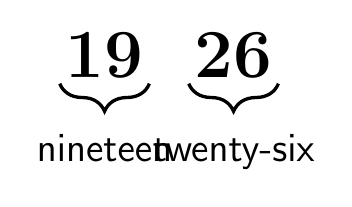
\begin{tikzpicture}[
            number/.style={
                font=\fontsize{60}{70}\selectfont\bfseries,
                inner sep=2pt,
                anchor=south west
            },
            label/.style={
                font=\Large\sffamily,
                anchor=north % 文字の上側を基準点にする
            },
            brace/.style={
                decorate,
                decoration={brace, amplitude=10pt, mirror},
                very thick
            }
        ]

            % --- Slide 1: 数字を表示 (<1-> 1枚目からずっと表示) ---
            
            \node<1->[number] (nineteen) at (0,0) {19};
            \node<1->[number, right=0.5cm of nineteen] (twentysix) {26};


            % --- Slide 2: 波かっこを表示 (<2-> 2枚目以降で表示) ---
            
            % 英語テキストと分離するため、ここでは draw コマンドのみにします
            \draw<2->[brace] (nineteen.south west) -- (nineteen.south east);
            \draw<2->[brace] (twentysix.south west) -- (twentysix.south east);


            % --- Slide 3: 英語を表示 (<3-> 3枚目以降で表示) ---
            
            % 波かっことは別のノードとして配置します。
            % 位置は「数字の下端(south)」から少し下(yshift)にずらした場所です。
            % 波かっこの深さ(10pt)より少し下になるように -15pt しています。
            
            \node<3->[label] at ([yshift=-15pt]nineteen.south) {nineteen};
            \node<3->[label] at ([yshift=-15pt]twentysix.south) {twenty-six};

        \end{tikzpicture}
    \end{overlayarea}
\end{frame}
%%%%%%%%%%%%%%%%%%%%%%%%%%%%%%%%%%%%%%%%%%%%%%%%%
\begin{frame}[plain]{Exercises}
 つぎの年号を英語で書きましょう

\visible<4->{yy00年~yy09年まではちょっぴり要注意}

\Large
\begin{enumerate}
 \item 1776\hfill\visible<2->{\makebox[80pt][l]{seventeen seventy-six}}\hspace{200pt}\mbox{}
 \item 1861\hfill\visible<3->{\makebox[80pt][l]{eighteen sixty-one}}\hspace{200pt}\mbox{}
 \item 1900\hfill\visible<5->{\makebox[80pt][l]{nineteen hundred}}\hspace{200pt}\mbox{}
 \item 1905\hfill\visible<6->{\makebox[80pt][l]{nineteen oh five}}\hspace{200pt}\mbox{}
 \item 1910\hfill\visible<7->{\makebox[80pt][l]{nineteen ten}}\hspace{200pt}\mbox{}
 \item 1998\hfill\visible<8->{\makebox[80pt][l]{nineteen ninety-eight}}\hspace{200pt}\mbox{}
\end{enumerate}
\end{frame}
%%%%%%%%%%%%%%%%%%%%%%%%%%%%%%%%%%%%%%%%%%%%%%%
\begin{frame}[plain]{Exercises}
\visible<3->{ややこしいのは2000年以降}

\Large
\begin{enumerate}
 \item 1999\hfill\visible<2->{\makebox[80pt][l]{nineteen ninety-nine}}\hspace{200pt}\mbox{}
 \item 2000\hfill\visible<4->{\makebox[80pt][l]{two thousand}}\hspace{200pt}\mbox{}
 \item 2003\hfill\visible<5->{\makebox[80pt][l]{two thousand three}}\hspace{200pt}\mbox{}
 \item 2009\hfill\visible<6->{\makebox[80pt][l]{two thousand nine}}\hspace{200pt}\mbox{}
 \item 2010\hfill\visible<7->{\makebox[80pt][l]{twenty ten\hspace{53.75pt}{\small (two thousand ten)}}}\hspace{200pt}\mbox{}
 \item 2020\hfill\visible<8->{\makebox[80pt][l]{twenty twenty\hspace{31.75pt}{\small (two thousand twenty)}}}\hspace{200pt}\mbox{}
 \item 2026\hfill\visible<9->{\makebox[80pt][l]{twenty twenty-six\hspace{5pt} {\small (two thousand twenty-six)}}}\hspace{200pt}\mbox{}
\end{enumerate}
\end{frame}
%%%%%%%%%%%%%%%%%%
\begin{frame}[plain]

 {\tiny audio\_overview 1208}\,{\scriptsize \myaudio{./audio/overview/014_when_audio_overview.m4a}}
\end{frame}
%%%%%%%%%%%%%%%%%%%%%%%%%%
\end{document}
